% Include this fragment from the paper root in an acmart document.
% Adjust the graphic path if the figure is stored elsewhere.
\begin{figure}[t]
  \centering
  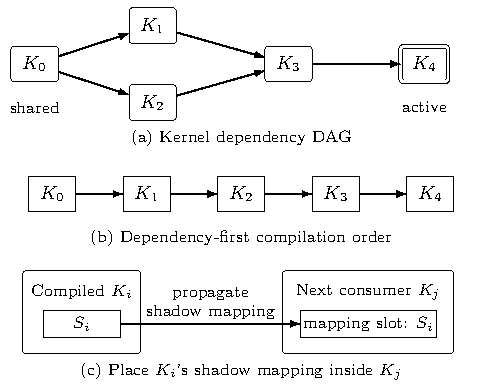
\includegraphics[width=\columnwidth]{docs/figures/dtl-dependency-dag.pdf}
  \caption{Dependency compilation of composed DTL kernels.
    (a) Edges point from a dependency to its consumer; the double-bordered
    node is the active kernel.
    (b) A valid topological compilation order visits each reachable kernel
    once, preserving the shared $K_0$ dependency.
    The independent kernels $K_1$ and $K_2$ may be compiled in either order.
    (c) The shadow mapping $S_i$ of a dependency $K_i$ is propagated into
    a mapping slot inside the next consuming kernel $K_j$.
    Propagation follows dependency edges, not mere adjacency in the compilation order.}
  \Description{Three panels. The upper graph has five nodes with directed
    edges from K0 to K1 and K2, from K1 and K2 to K3, and from K3 to K4.
    The middle panel is a left-to-right sequence of K0, K1, K2, K3, and K4.
    The lower panel shows a compiled kernel Ki containing shadow mapping Si.
    An arrow labeled propagate shadow mapping ends at a mapping slot containing
    Si inside the box for the next consuming kernel Kj.}
  \label{fig:dtl-dependency-dag}
\end{figure}
